\documentclass[TeXworkshop]{subfiles}
\begin{document}
\clearpage

\section{\TeX のすゝめ}
ここで,本章でやることの概要を書く.

\subsection{ワープロソフトの種類}
動作に着目すると、文書を作成するソフトウェアは大きく2タイプに分類することができます。
1つは、テキストの編集画面をほぼそのまま出力する\ruby{WYSIWYG}{ウィジウィグ}
[What You See Is What You \kenten{G}et]タイプ、
% フリガナ追加
もう1つは、文書の構造を明示的に定義して編集を行う
\ruby{WYSIWYM}{ウィジウィム} [What You See Is What You \kenten{M}ean]タイプです。

私たちは、日々の研究活動や業務において様々な種類の文書を扱いますが、
その特性の大部分は文書の規模、構造化の程度や内容の反復度、
数値データの数、相互参照や図表の数などによって決定されます。
品質要求を満たした文書を最短時間で作成するためには、
自身が作成しようとしている文書の特性を見極め、
適切なタイプのソフトウェアを使用する必要があります。
それでは、これら2つのタイプの文書作成ソフトウェアは、どのように異なるのでしょうか。

\subsubsection{WYSIWYG}
WYSIWYGタイプのソフトウェアの中にも、シンプルなものから高機能なものまで様々ありますが、
ある程度の規模の文書を作成する場合には、
Microsoft Wordのように、図表の挿入から校正機能など、
多くの機能を備えた「オール・インワン」的なソフトウェアを使用することが多いようです
(表 \ref{table:differences})。
これらはマウスを用いた直感的な操作性に優れているため、
使用開始初期の学習コストが低いのが特長です。


\subsubsection{WYSIWYM}
本講習では、このWISIWIMタイプのソフトウェアの代表格である\TeX について学びます。
本来、両タイプのソフトウェアの性能には一概に優劣をつけられるものではありませんが、
私たち研究者が業務で作成する文書の大部分が、図表や文献を多く含み、高度に構造化されていることを考えれば、
私たちが\TeX を学ぶことのメリットは十分に大きいと言えます。

WYSIWYMタイプのソフトウェアでは、編集画面が見たままに出力されないため、
文書内の図表などの要素の位置をテキストで細かく指定したり、文章にさまざまな属性を与えることができます。
本講習で紹介する\TeX は、このWYSIWYMタイプのソフトウェアの代表格です。


\TeX では、目次や図表、索引、脚注、数式番号、文献などの参照も、
ファイル名や参照のための手がかりを埋め込んでおくことによって、容易に実現できます。
「○○ページを御覧ください」のような、特定ページの参照も可能です。
この方式をとっていることによって、\TeX で作成された文書は変更に強く、再現性を高く保つことができます
(表 \ref{table:differences})。
文書の体裁に注意力を削がれずに済むため、執筆者は残りの作業時間の大部分を文書内容の推敲に充てることができます。

\TeX は、変更を成果物に反映させるためにコンパイルを必要とします。
この作業によって、文書ファイル内に埋め込まれた体裁に関する命令や、
相互参照の手がかりを拾い集め、最終的な成果物を作成します。
コンパイルは一見、煩わしい手間に思えるかもしれませんが、\TeX はユーザーからの入力を常時監視せずに済みますし、
編集する文書自体はタネも仕掛けもない単なるプレーンテキストですので
\footnote{例えばMS Wordの \ttfamily{.docx}ファイルは仕掛けだらけで、\\
本文が記述されたファイルの他に、様々な設定やコンテンツファイル群がまとめられていますが、\\
それらはあたかも一つのファイルであるかのように隠蔽されています。}、
大規模な文書を扱う際にも動作を軽快に保つことができます。

\begin{table}[h]
 \begin{center}
  \caption{Microsoft Wordと\TeX の長所の違い}
  \label{table:differences}
  \begin{tabular}{rcc}
   & Word & \TeX \\\hline
   機能の数              & $\circ$ & $\times$\\
   直感的操作            & $\circ$ & $\times$\\
   学習コスト            & $\circ$ & $\times$\\
   再現性                & $\times$ & $\circ$ \\
   相互参照              & $\times$ & $\circ$ \\
   大規模文書の扱いやすさ& $\times$ & $\circ$ \\\hline
  \end{tabular}
 \end{center}
\end{table}

\begin{itembox}[l]{メモ}
 \TeX の隠れた特長に、仕上がりの美しさが挙げられます。
 これは、\TeX が単なるワープロソフトではなく、
 美しい文書を作成することを目的として開発された「組版」ソフトであるためです。
 \TeX の開発者であるDonald Knuth博士は、自著をあたかも組版職人によって組版されたかのように
 美しく仕上げたいと考え、1976年に\TeX の開発を始めました。
\end{itembox}


\subsection{報告書・論文作成には\TeX を}
WYSIWIG/WYSIWYM両タイプのソフトウェア(以下Microsoft Wordと\TeX)は
場面に応じて適切に使い分けることが重要です。
このことを理解するために、万能包丁と蕎麦切り包丁のアナロジーを考えてみましょう。
料理(文書)の特性に合わせて、包丁(ソフトウェア)を使い分けるのは自然なことです。

ちょっと小腹が空いてしまった状況を考えてみましょう.
自分で食べるちょっとした一皿を、冷蔵庫にあるあり合わせの材料で、
手早く美味しく作りたい...
この状況で、蕎麦切り包丁を手にする人はいないでしょう。
こんな時には万能包丁の出番です。

では、あなたがお蕎麦屋さんの蕎麦打ち職人だったらどうでしょうか。
とびきり美味しい蕎麦を食べてもらいたいと思っているのに,
まして太さがバラバラの麺をお出しするわけには行きませんよね.
麺を真っ直ぐ切る仕事は蕎麦切り包丁に任せ,あなたは麺の味わいやコシを追求することに集中すべきです.
間違っても,万能包丁を手に四苦八苦してはいけません.

「ちょっとした一皿と万能包丁」はちょっとした覚え書きとMicrosoft Wordの、
「自慢の蕎麦と蕎麦切り包丁」は報告書や学術論文と\TeX のアナロジーです。
毎年、一定のフォーマットで提出する報告書、IMRAD型式の学術論文は、\TeX で作成しましょう。

\subsection{\TeX ファイルの構造}
\TeX で文書を作成するための\ttfamily{.tex}ファイルは大まかには2つの部分に分かれています。
1つは文書の構造や仕様を定義するための「プリアンブル」、
もう1つは実際に印刷される内容を執筆するための「ドキュメント」です(図\ref{fig:example_wagahai})。
それぞれの役割を見ていきましょう。

\begin{figure}[H]
 \begin{center}
  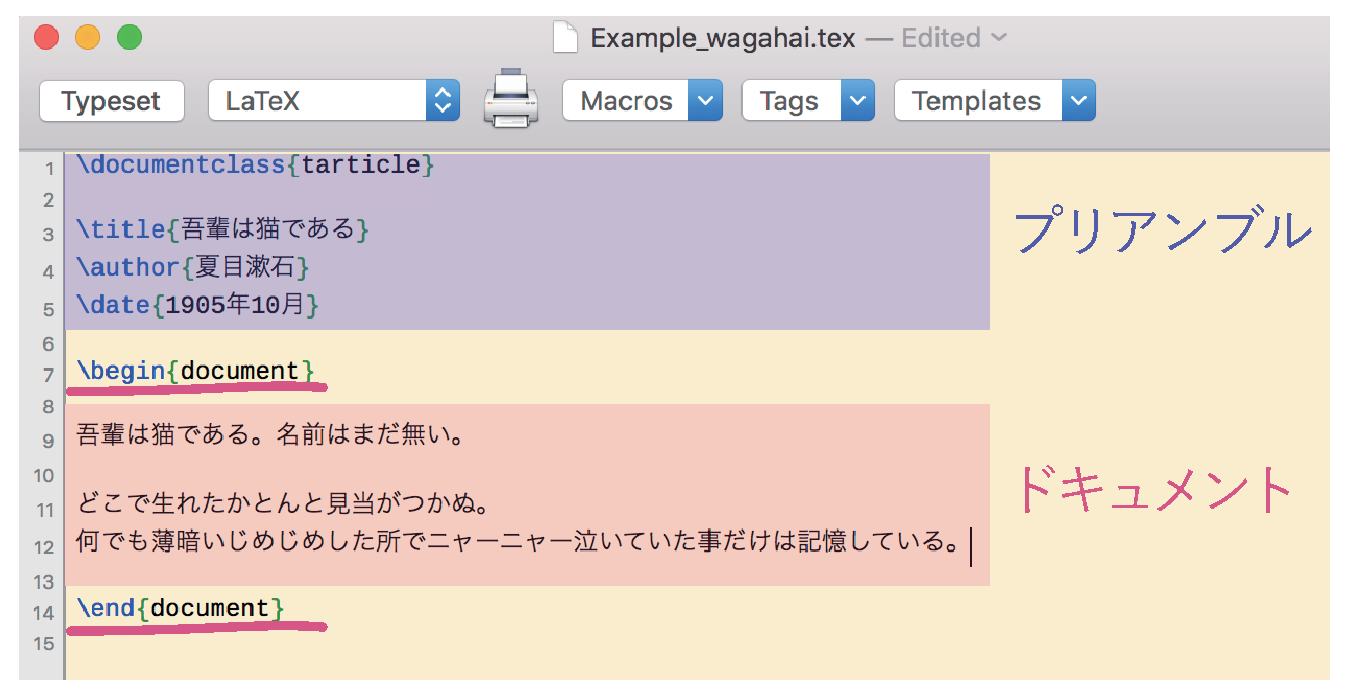
\includegraphics[width=\textwidth,clip]{Example_wagahai.eps}
  \caption{test}\label{fig:example_wagahai}
 \end{center}
\end{figure}

\subsubsection{プリアンブル}
\ttfamily{.tex}ファイルを開いて最初に目に入る先頭部分がプリアンブルです(図\ref{fig:example_wagahai}の青色部分)。
プリアンブルは、その文書をどのような形の媒体で印刷するのかを設定する場所です。
図\ref{fig:example_wagahai}の1行目に書かれている
\verb|\documentclass{tarticle}|は、「この文書を縦書きのarticle型式の文書クラスで出力せよ」という命令です。
この\ttfamily{.tex}ファイルをコンパイルすると、図\ref{fig:tategaki}のような文書が出力されます。

\begin{figure}[H]
 \begin{center}
  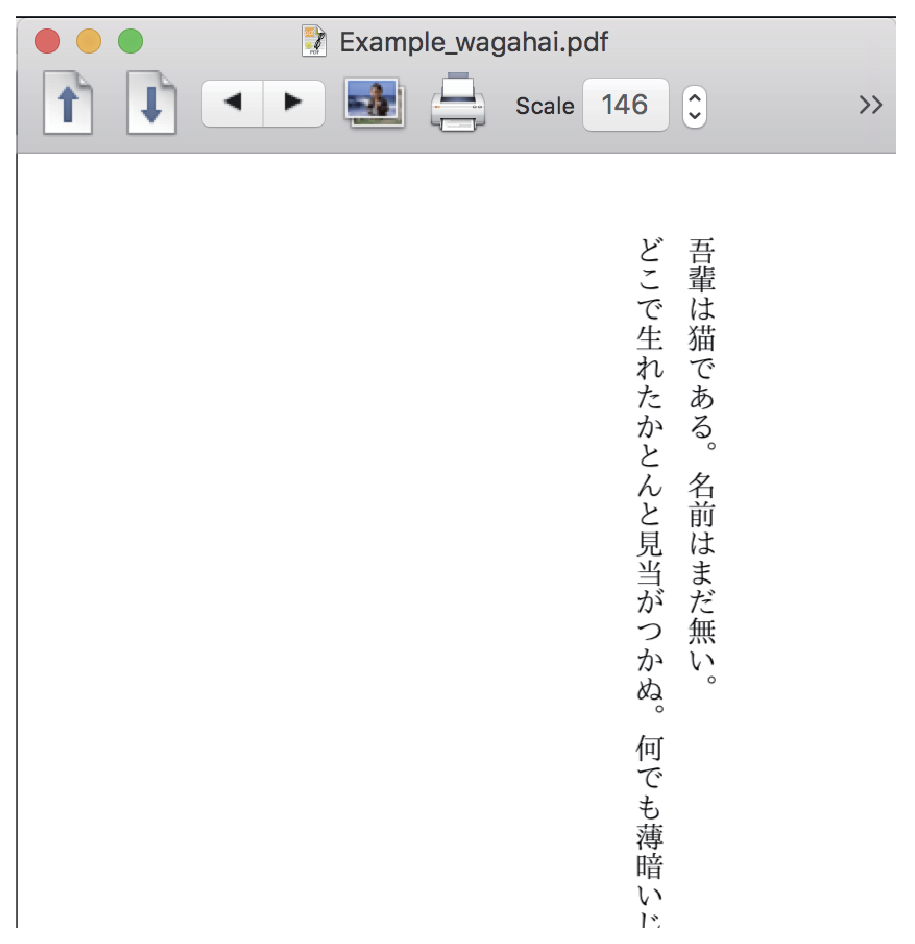
\includegraphics[width=0.5\textwidth,clip]{tategaki.eps}
  \caption{test}\label{fig:tategaki}
 \end{center}
\end{figure}


小説らしいレイアウトですね。

ここで、プリアンブルの役割を理解するために、文書クラスを\ttfamily{"article"}に変更してみましょう(図\ref{fig:change_doc_class}(a))。
コンパイルしてみると、図\ref{fig:change_doc_class} (b) のように、ただちに横書きの文書が出力されます。
\begin{figure}[htbp]
 \centering
 \subfigure[\ttfamily{.tex}ファイル]{
 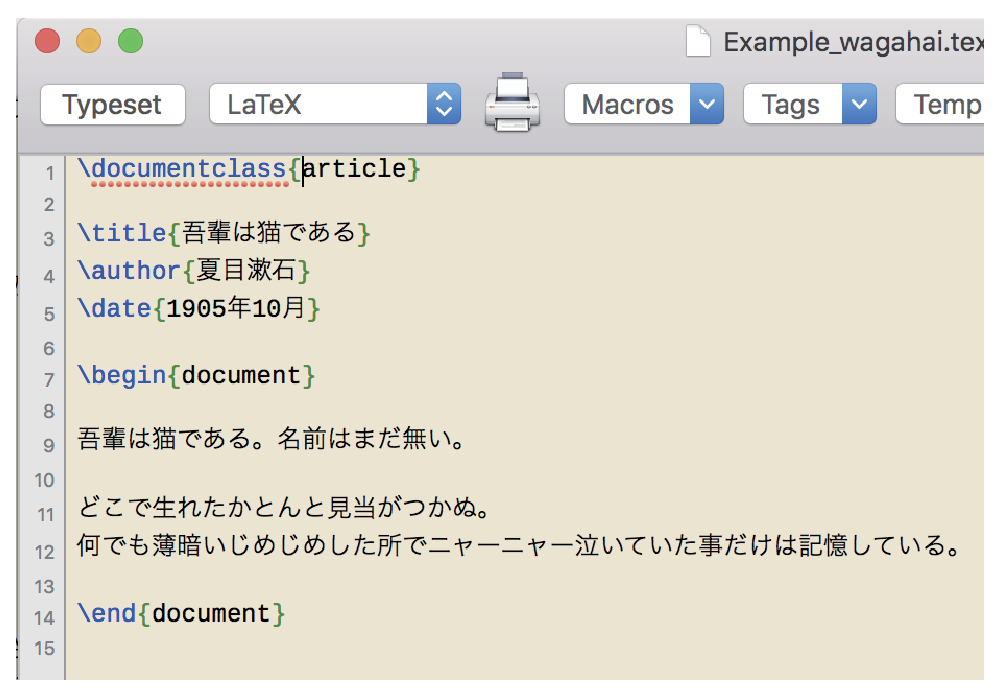
\includegraphics[clip, width=0.45\textwidth]{yokogaki.eps}
 \label{fig:yokogaki_src}
 }
 \subfigure[出力]{
 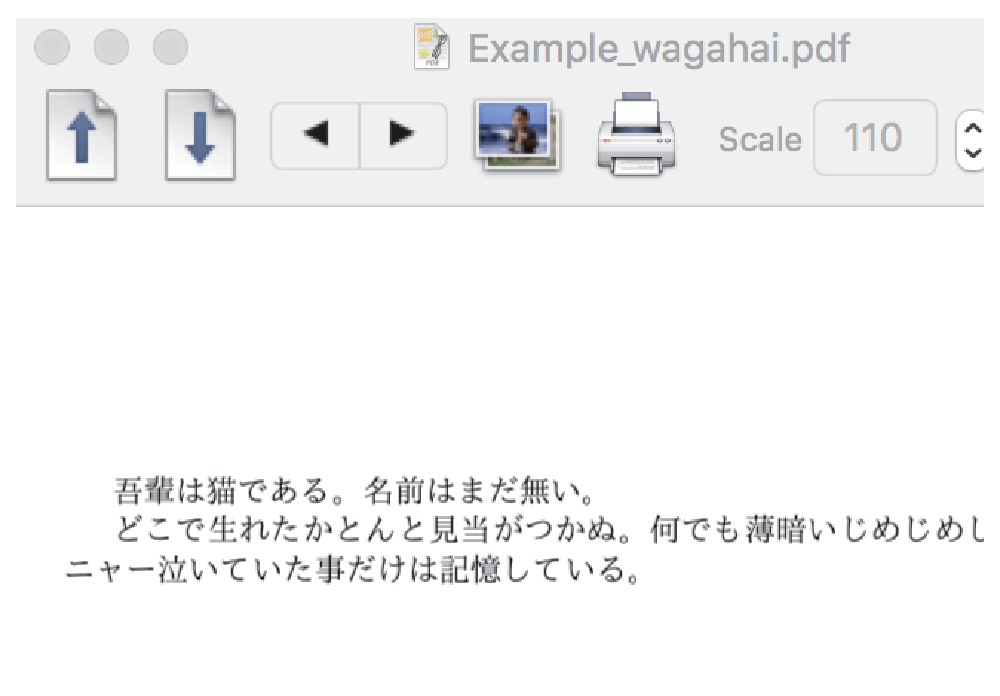
\includegraphics[clip, width=0.45\textwidth]{yokogaki_output.eps}
 \label{fig:yokogaki_out}
 }
 \caption{文書クラスの変更例}
 \label{fig:change_doc_class}
\end{figure}



このように、文書の仕様を指定するのがプリアンブルの役目です。




\subsubsection{ドキュメント}

\verb|\begin{document}|と\verb|\end{document}|に挟まれた部分を「ドキュメント」と呼びます。
実際の執筆作業のほとんどはこの部分で行います。

本文の執筆中、特定の箇所で書式を変更する必要が生じた場合、
\TeX では、バックスラッシュ(\textbackslash)\footnote{Windows環境の場合は円通貨記号}
や中括弧を用いた
「関数」を用いる決まりがあります。

「章」「節」などの文書の構造に関わる見出し
\footnote{
part、chapter、section、subsection、subsubsection、paragraph、subparagraph
などが利用可能です}
は、
\verb|\chapter{章の名前}|
\verb|\section{節の名前}|
などのように指定する決まりがあり、
それぞれのレベルに予め設定された書式が自動的に適用されます。

文書の構造に関係がない部分に書式を変更したい場合にも、
やはり関数が必要です(図\ref{fig:large_italic})。
しかし、ドキュメント部でその都度関数を呼び出し、
書式をその場限りで変更するこのような方法は、
\TeX では推奨されていません。
それはなぜでしょうか。

\begin{figure}[htbp]
 \centering
 \subfigure[\ttfamily{.tex}ファイル]{
 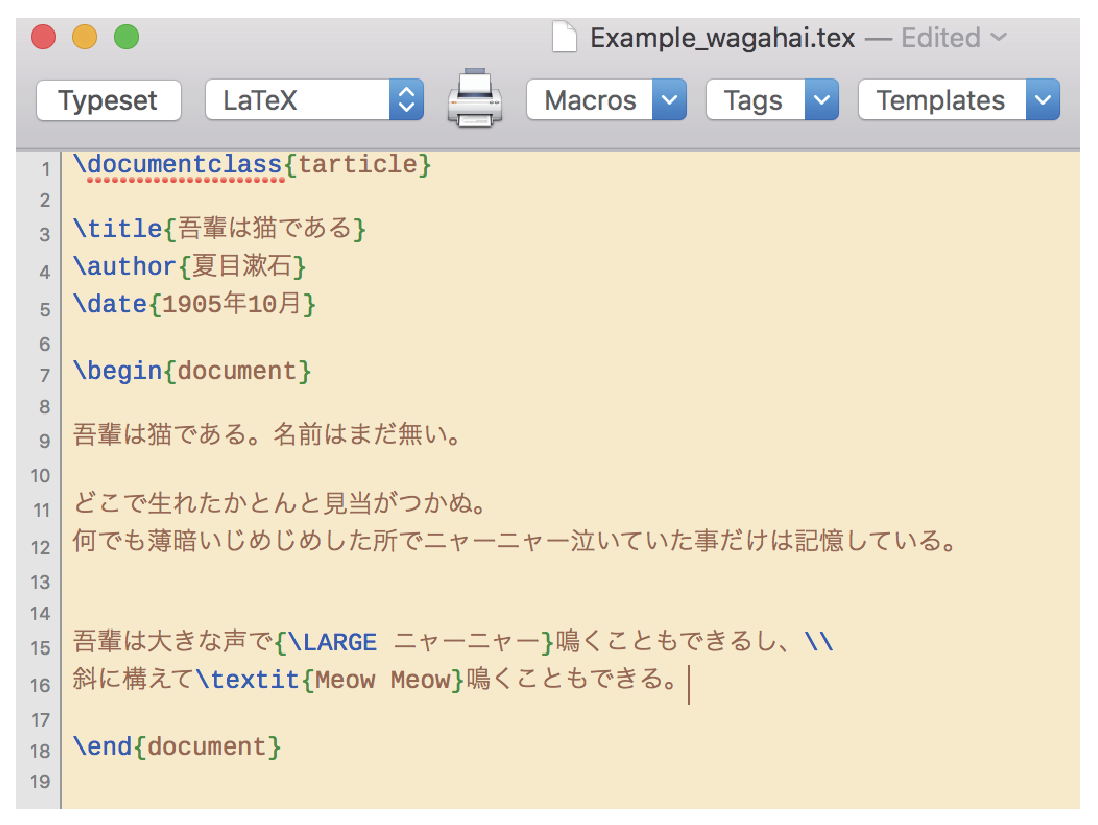
\includegraphics[clip, width=0.45\textwidth]{large_italic.eps}
 \label{fig:large_italic_src}
 }
 \subfigure[出力]{
 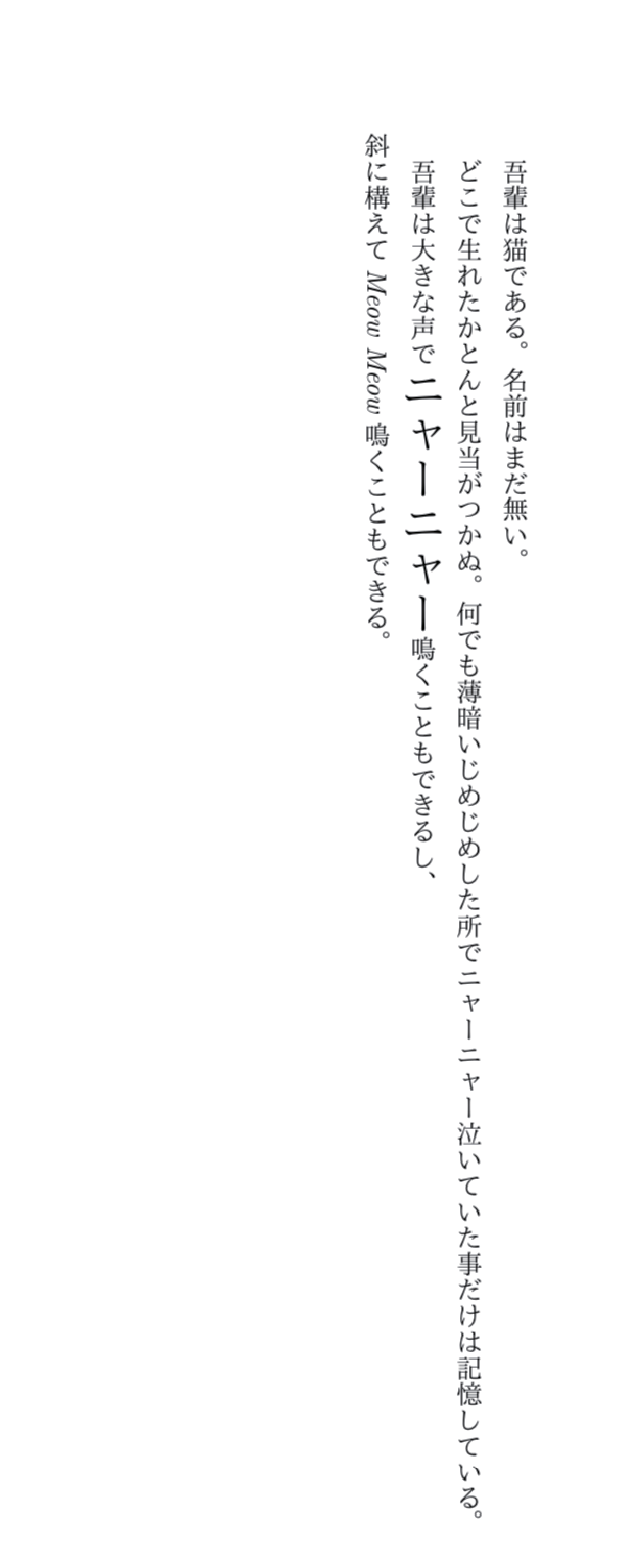
\includegraphics[trim={3cm 7cm 0 0},clip, width=0.3\textwidth]{large_italic_out.eps}
 \label{fig:large_italic_out}
 }
 \caption{その場限りのフォント変更}
 \label{fig:large_italic}
\end{figure}
\clearpage

\subsubsection{\TeX らしい記法: マクロ}
文字を大きくしたい箇所が文書中に複数箇所ある場合を考えてみます(図\ref{fig:redundant})。
\verb|{\LARGE ニャーニャー}|という面倒なタイピングを、
本文中であと何回繰り返すことになりそうでしょうか。
もし、この部分のフォントのサイズを変更したくなったら、
検索・置換作業を繰り返し、サイズ指定を変更して回らねばなりません。

\begin{figure}[htbp]
 \centering
 \subfigure[\ttfamily{.tex}ファイル]{
 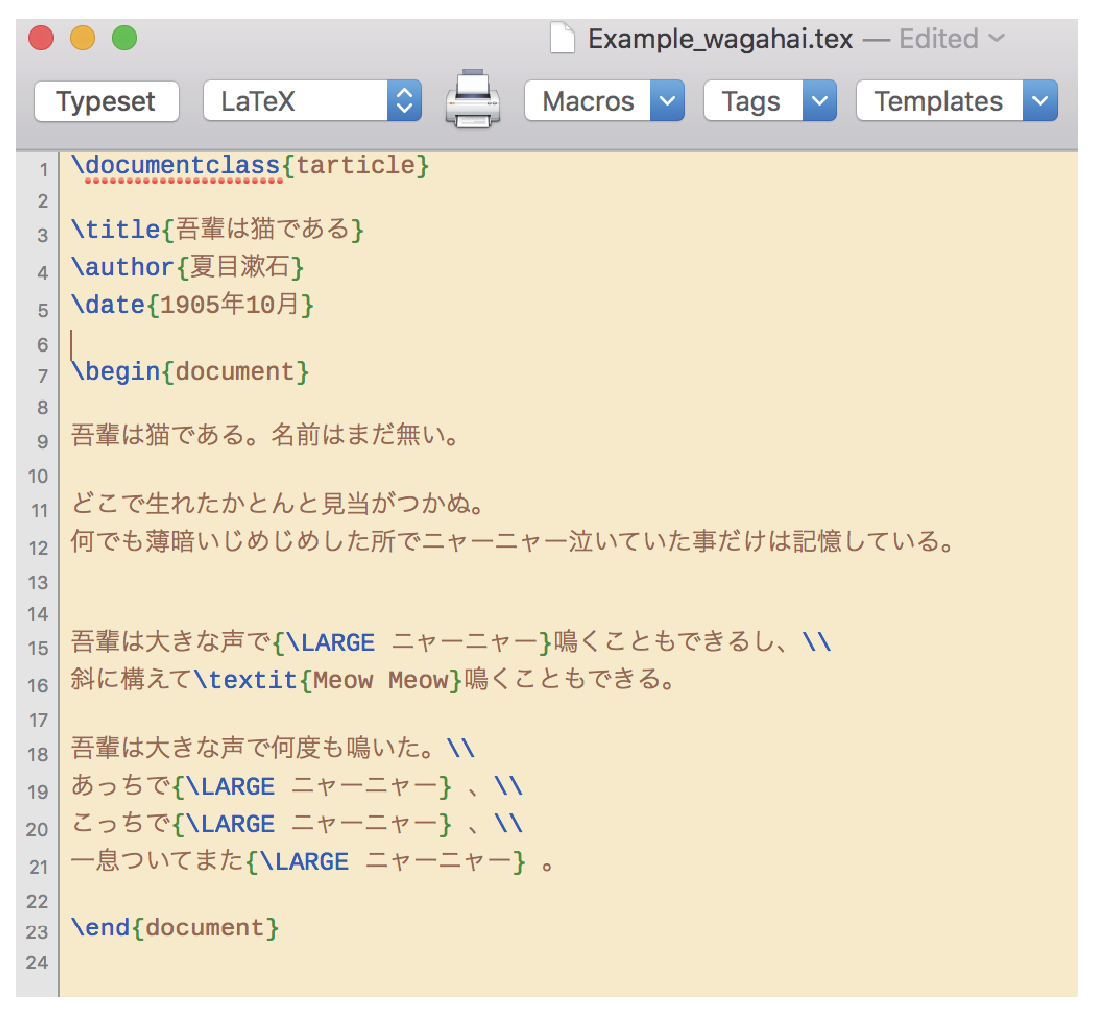
\includegraphics[clip, width=0.45\textwidth]{redundant.eps}
 \label{fig:redundant_src}
 }
 \subfigure[出力]{
 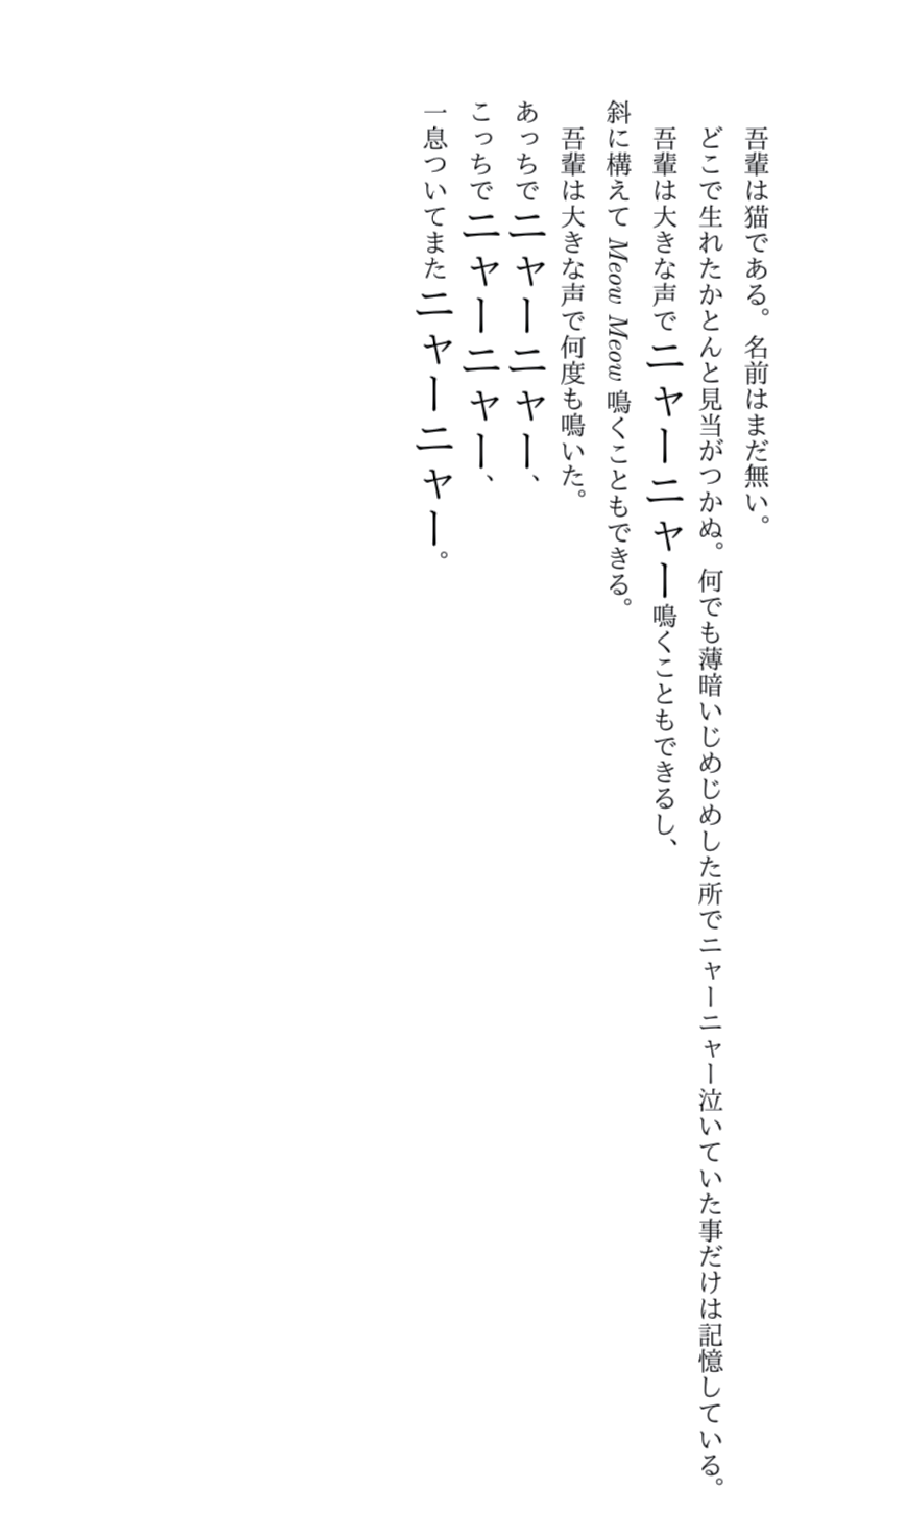
\includegraphics[clip, width=0.45\textwidth]{redundant_out.eps}
 \label{fig:redundant_out}
 }\caption{そのばしのぎはあとが大変}
 \label{fig:redundant}
\end{figure}

このような状況を回避するために、
\TeX ではプリアンブルにおけるマクロの定義(図\ref{fig:macro})が推奨されています。
\begin{figure}[htbp]
 \centering
 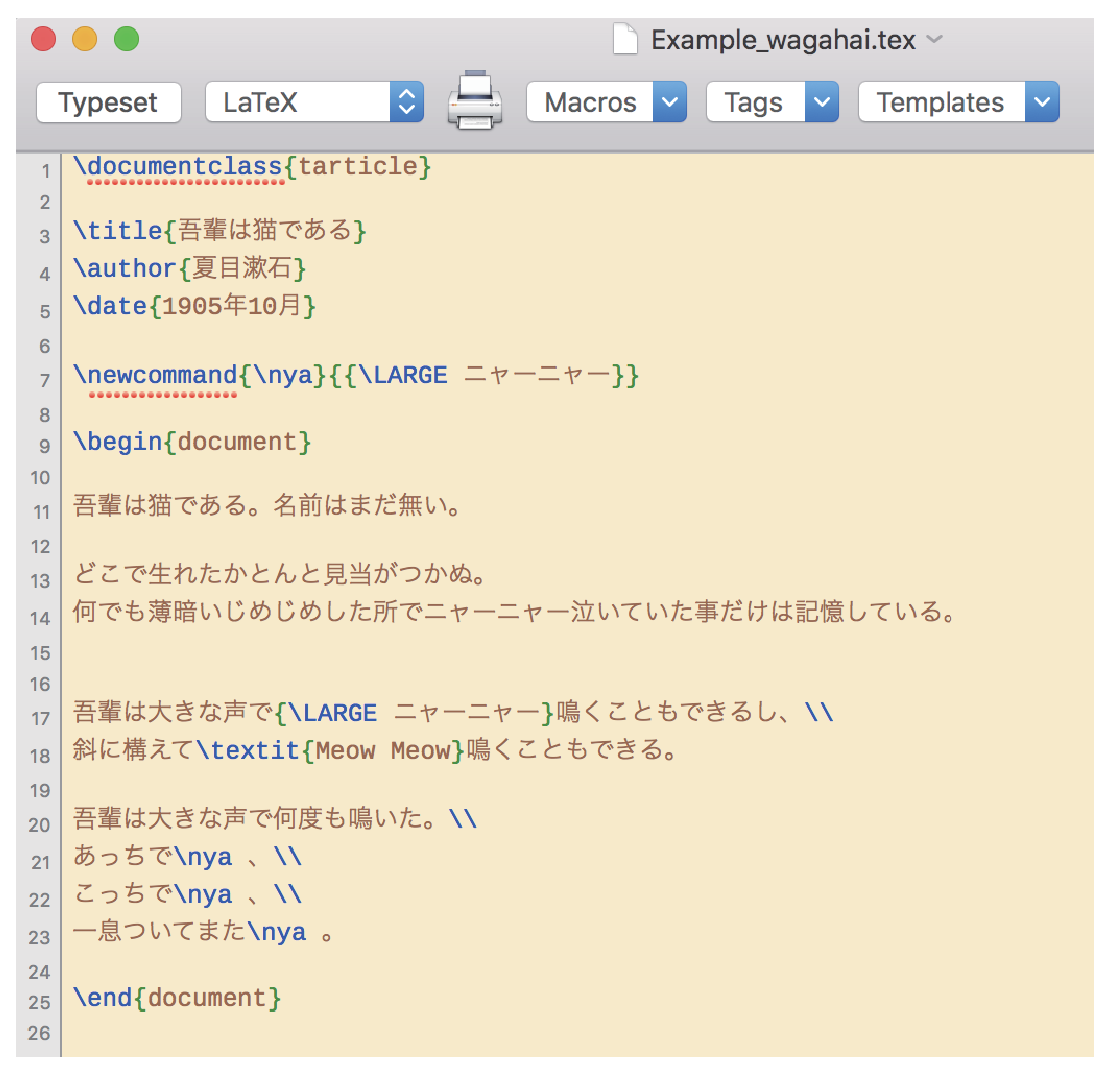
\includegraphics[clip, width=\textwidth]{macro.eps}
 \caption{マクロを利用したフォントの変更}
 \label{fig:macro}
\end{figure}
マクロはひとたび定義してしまえば、本文中で呼び出すことによって何度でも利用でき、
何よりもプリアンブルにおける定義を変更するだけで一括で設定を変更できるのが利点です。

\TeX の具体的な使い方を学ぶには、実際にコードの編集とコンパイルを繰り返すのが一番です。
本講習で配布するサンプルコードで、いろいろと試してみてください。

\begin{itembox}[l]{コラム: \TeX 記法は面倒?}
 本文のフォントや体裁を変更する場合、
 「気軽さ」という観点では、\TeX はMS Wordには到底敵いません。
 MS Wordではキーボードショートカットで瞬時に作業が完了するのに対し、
 \TeX の関数は、入力に時間がかかる上、入力後も本文中でスペースを占め続けます。
 このように、\TeX 記法は一見、時空間的コストが高く思えるのですが、
 この特性は文書の規模が大きくなるにつれ、むしろメリットに変化していきます。

 体裁の指定が目立つこと自体が、1つ目のメリットといえるでしょう。
 体裁の指定が目立つ分、単純に、体裁の直し忘れが起こりにくいですし、プレーンテキストなので検索も可能です。

 2つめのメリットはさらに重要です。
 \TeX 記法は体裁の指定に手間がかかる分、自分が今から\kenten{何をしようとしているのか}を、慎重に考えるようになります。
 例えば、フォントの色や大きさを変えようとしているとき、その本来の目的はその部分を強調して伝えることでしょう。
 ひょっとしたら、フォントを変更して文面を煩雑にするよりも、アウトラインを整理する方がよほど効果的かもしれません。

\end{itembox}

\begin{itembox}[l]{コラム: タイトル}
 ここまで示してきた図のプリアンブルに、
 \verb|\title{吾輩は猫である}|
 や
 \verb|\author{夏目漱石}|
 などと書いてあったのにお気づきでしたでしょうか。
 これは\TeX に標準で備わった、文書の情報(属性といいます)を格納するマクロの一種です。
 ドキュメント部に\verb|\maketitle|と書けば、
 著者名や表題、日付が書かれたタイトルページが出力されます。
\end{itembox}

\subsection{本章で学んだこと}
\begin{itemize}
  \item WISIWIG と WISIWIM 方式の違いと,それぞれの得意とする作業
  \item 報告書に適しているのは WISIWIM 方式で,\TeX はその代表格である
  \item \TeX らしい記法の紹介
\end{itemize}



\end{document}
